\chapter{ПЕРЕДАЧА ВИДЕОИНФОРМАЦИИ В БЕСПРОВОДНЫХ ЦЕНТРАЛИЗОВАННЫХ СЕТЯХ}
\label{chap2}

\section{Вводные замечания}
\label{chap2:Intro}

Оптимизация передачи видеоинформации наиболее актуальна для беспроводных систем связи по причине наличия ограничений на пропускную способность радиоканала, который считается <<узким местом>> (адаптированный перевод англоязычного термина <<bottle neck>>) сети в целом. Основная проблематика всех исследований в области передачи видеоинформации состоит не в предложении методов управления для телекоммуникационных сетей, а в обосновании их эффективности. Любое возможное управление может увеличить производительность системы, используя дополнительную информацию о передаваемом контенте, однако, в настоящее время не существует опорных теоретических исследований, с которыми возможно сравнить производительность предлагаемых решений. Данная диссертационная работа ставит перед собой задачу предложить границы, характеризующие максимально возможную производительность мобильных сетей для передачи видеоинформации.

Настоящий раздел посвящен задаче передачи видеоинформации в современных мобильных централизованных сетях. В разделе рассматривается специфика построения современных мобильных сетей связи, и решается задача формирования аналитической модели для проведения исследований подобных систем при передаче видеоинформации. В начале производится обзор структуры и важных элементов мобильных сетей на основе современного стандарта передачи информации The Long-Term Evolution (LTE). Далее предлагается аналитическая модель, которая включает в себя все компоненты системы и позволяет провести строгие теоретические исследования передачи видеоинформации через мобильные сети. Для введенной модели предлагается основополагающая лемма, описывающая взаимосвязь между всеми характеристиками сети, влияющими на ее производительность. В заключении данного раздела предлагается анализ полученной леммы.

Основные результаты данного раздела опубликованы в работах...

Ввиду большого объема англоязычных терминов, использованных при описании стандарта LTE ниже приведен список аббревиатур и краткое описание англоязычных терминов.
\begin{itemize}
  \item The Long-Term Evolution (LTE)~--~стандарт передачи информации в беспроводных централизованных сетях;
  \item Internet Protocol (IP)~--~протокол сетевого уровня, обеспечивающий маршрутизацию в сети;
  \item Application Layer (APP)~--~обозначение уровня приложения в семиуровневой модели;
  \item Physical Layer (PHY)~--~обозначение физического уровня в семиуровневой модели;
  \item Media Access Control (MAC)~--~обозначение уровня доступа ко среде в семиуровневой модели;
  \item User Datagram Protocol (UDP)~--~протокол транспортного уроня;
  \item GPRS Tunneling Protocol (GTP)~--~протокол обеспечивающий маршрутизацию в опорной сети оператора;
  \item Packet Data Convergence Protocol (PDCP)~--~протокол радиосети стандарта LTE, обеспечивающий целостность передачи информации через радиосеть;
  \item Radio Link Control (RLC)~--~протокол радиосети стандарта LTE, обслуживающий очереди данных при передаче через радиосеть.
\end{itemize}

\section{Структура современных беспроводных централизованных сетей передачи информации}
\label{chap2:WirelessSystemStructure}

В настоящее время существующие мобильные системы передачи информации разделяются на три основных компонента (рисунок~\ref{fig:LteStructure}):
\begin{itemize}
  \item Фиксированная магистральная сеть передачи данных. Сеть передачи информации, в которая обеспечивает соединение с удаленными устройствами (в системах передачи видеоинформации таким устройством является Видео Контент Сервер). Она характеризуется высокой надежностью, большой скоростью передачи информации, низкими задержкой и джиттром.
  \item Опорная сеть оператора (Core Network или Evolved Packet Core). Система устройств, обеспечивающая взаимодействие мобильного пользователя с удаленными устройствами в фиксированной магистральной сети. Обладает схожими характеристиками с магистральной сетью.
  \item Радиосеть. Беспроводная сеть передачи информации, организующая обмен данными между мобильным устройством и остальными компонентами сети. Характеризуется несравнимо меньшими скоростями передачи информации и пропускными способностями каналов, большими задержкой и джиттером. Важной отличительной особенностью радиосети является изменяемость состояний каналов передачи информации во времени.
\end{itemize}

\begin{figure}[htbp]
\begin{center}
\includegraphics[width=\textwidth,height=0.4\textheight]{Chapter2/LteStucture.pdf}
\caption{Структура современных беспроводных централизованных систем}
\label{fig:LteStructure}
\end{center}
\end{figure}

На текущий момент времени наибольшее распространение получили централизованные мобильные сети, так как они обеспечивают наиболее высокие скорости и малую задержку при передаче информации~\cite{Cisco}. Важным отличием централизованных беспроводных систем является наличие устройства, управляющего передачей информацией всех активных пользователей в его зоне ответственности (для централизованных сетей территория обслуживания разделена на участки, называемые сотами), называемого Базовой станцией. Базовая станция~--~программно-аппаратный комплекс обеспечивающий обмен информацией между пользователем в радиосети и опорной сетью оператора.

Последним этапом развития современных мобильных централизованных систем связи является стандарт The Long-Term Evolution (LTE), иногда называемый стандартом четвертого поколения (4G) мобильных сетей. Стандарт LTE был спроектирован как полностью пакетно-ориентированная система, в отличии от стандартов предыдущего поколения. Важным нововведением данного стандарта является появление <<носителя>> (в англоязычной литературе Bearer)~--~абстрактное представление взаимосвязи между пользователем, видом используемого трафика и требованиями к его обслуживанию. Например, когда упоминается видео носитель пользователя, то подразумевается какие характеристики соединения: максимальная и минимальная скорость получения информации, задержка и т.д., должны быть обеспечены данному конкретному пользователю при использовании видео трафика. Для одного пользователя может быть несколько носителей. Данное нововведение обеспечило увеличение производительности сети, по сравнению с предыдущими стандартами связи~\cite{opac-b1130916}.

Так как стандарт LTE получил широкое распространение и постоянно развивается, в данной работе он был принят в качестве опорного для построения аналитической модели. Для полноценного введения и обоснования системы принятых допущений аналитической модели системы передачи видеоинформации через мобильные сети необходимо представить описание функций опорной сети оператора и радиосети. Данный обзор предоставлен в подразделах \ref{chap2:CoreNetwork} и \ref{chap2:RadioNetwork}, аналитическая модель представлена в подразделе~\ref{chap2:AnalyticalModel}.

Работу мобильной сети в целом обеспечивает стек протоколов передачи информации, представленный на рисунке~\ref{fig:LteProtocolStack}.

\begin{figure}[htbp]
\begin{center}
\includegraphics[width=\textwidth,height=0.4\textheight]{Chapter2/LteProtocolStack.pdf}
\caption{Стек протоколов, обеспечивающий передачу информации в стандарте LTE}
\label{fig:LteProtocolStack}
\end{center}
\end{figure}

\section{Передача информации через опорную сеть оператора}
\label{chap2:CoreNetwork}
Опорная сеть оператора явлется важными компонентом сети передачи информации, отвечающим за организацию обмена информацией с фиксированной магистральной сетью. Важнейшие функциональные компоненты сети оператора представлены в списке ниже:
\begin{itemize}
  \item Узел управления мобильностью (Mobility Management Entity или MME)~--~основной узел, управляющий работой сети оператора в целом. Выполняет следующие функции:
  \begin{itemize}
  	\item Идентификация и авторизация пользователя при подключении к сети оператора;
  	\item Установка пользователям носителей, исходя из тарифной политики оператора;
  	\item Взаимодействие с сетями предыдущего поколения для обратной совместимости.
  \end{itemize}
  \item Обслуживающий шлюз (Serving Gateway). Обеспечивает сохранность информации при перемещении абонентов между базовыми станциями и взаимодействие с другими технологиями мобильной связи GPRS3 и UMTS;
  \item Пакетный шлюз (Packet Gateway) отвечает за маршрутизацию данных между пользовательским устройством и внешней сетью (управление IP~-~адресацией), фильтрацию пакетов из магистральной сети в различные носители на основе анализа трафика. Обеспечивает взаимодействие с технологиями CDMA2000 и WiMAX.
  \item Узел выставления счетов абонентам (Policy and Charging Rules Function) хранит соответствие тарифной политики оператора и пользователя. Данный узел имеет большое влияние на передачу информации через мобильную сеть, так как в зависимости от его решений изменяется приоритет обслуживания абонентов в радиосети.
\end{itemize}
Для наглядного объяснения логики передачи информации в опорной сети оператора необходимо рассмотреть доставку пакетов к пользовательскому устройству через опорную сеть оператора. Считается, что пользователь прошел все процедуры подключения к базовой станции, и вся необходимая информация имеется на основных узлах опорной сети. Важно отметить, что в централизованных беспроводных системах, и в частности стандарте LTE, пользователь подключен и обслуживается только одной базовой станции.

В опорной сети пользователь идентифицируется уникальным номером International Mobile Subscriber Identity (IMSI), который записан в сим-карте, выданной оператором мобильной связи. На основе идентификатора IMSI производится маршрутизация данных. Изначально пакет, предназначающийся для пользователя в радиосети, обрабатывается пакетным и обслуживающим шлюзами, которые определяют по IP адресу получателя его IMSI и базовую станцию, к которой он подключен. Важнейшей функцией пакетного шлюза явлется анализ трафика, проходящего через него, на основе данного анализа каждый пакет <<окрашивается>> в зависимости от вида трафика и распределяется по носителям. В настоящее время функциональные возможности пакетного шлюза совершенствуются по средствам дополнительного анализа системами Deep Packet Inspection (DPI), позволяющими получить больший объем информации о трафике абонента, например, для видеотрафика существует возможность дополнительно определить битовую скорость видеопотока для незашифрованного соединения. Маршрутизация в опорной сети производится на основе протокола туннелирования GPRS Tunneling Protocol (GTP), основанного на протоколе транспортного уровня User Datagram Protocol (UDP) (рисунок~\ref{fig:LteProtocolStack}). По средствам GTP протокола пакет доставляется на базовую станцию, где, пройдя через стек радио протоколов, будет доставлен на пользовательское устройство. При получении пакета на пакетном шлюзе о данном событии уведомляется узел выставления счетов абонентов, в зависимости от текущего статуса абонента узел может принять решение о изменении параметров носителей для пользователя, и как следствия приоритета его обслуживания.

Существуют проекты, которые ставят перед собой задачу оптимизации передачи видеоинформации в опорной сети оператора, путем получения информации от основных компонентов сети (Узлов управления мобильности, выставления счетов абонентам и шлюзов), и на основе полученной информации производить управления потоками для предотвращения перегрузок в радиосети~\cite{MobiVita}. Основной проблемой подобных проектов является ограниченный набор информации доступный для анализа. Он включает в себя лишь информацию доступную на сетевом уровне и выше, однако, из-за специфики беспроводного канала, сформировать своевременное и эффективное решение по оптимизации передачи видеоинформации без информации о характеристиках беспроводного канала является практически неразрешимой задачей.

Как следствие, наибольшее развитие получила ветвь исследований о управлении передачей видеоинформации на базовой станцией. На базовой станции дополнительно к набору информации, доступной в опорной сети оператора, имеется информация о характеристиках беспроводного канала, что позволяет организовать эффективное управление передачей данных.

\section{Организация передачи информации через радиосеть}
\label{chap2:RadioNetwork}

Основной задачей стека протоколов радиосети, представленной на рисунке~\ref{fig:LteProtocolStack}, является организация надежной передачи информации по ненадежному радиоканалу. Для решения данной задачи был разработан комплекс протоколов канального уровня и новый компонент базовой станции: планировщик ресурсов беспроводного канала (в англоязычной литературе используется обозначение Media Access Channel Scheduler или MAC Scheduler). Далее в работе для сокращения объема текста в качестве обозначения <<планировщика ресурсов беспроводного канала>> будет использоваться термин <<планировщик>>.

Изначально будет описано представление ресурсов и структура беспроводного канала на качественном уровне (рисунок~\ref{fig:LteRadioChannel}). В стандарте LTE на физическом уровне беспроводного канала все время разделено на периоды равной длины, называемые кадрами (в англоязычной литературе Frame) длительностью 10 миллисекунд, каждый кадр разделен на 10 подкадров (Subframe) длительностью 1 мс. В частотной области произведено разделение частотных ресурсов на области шириной 180 кГц, например, для ширины полосы 1 МГц полоса будет разделена на 5 областей (рисунок~\ref{fig:LteRadioChannel}). Минимальной единицей частотно-временных ресурсов является Ресурсный Блок~--~одна область шириной 180 кГц длительностью 1 мс. Ресурсные блоки относятся к общему каналу передачи информации, ресурсы которого могут быть распределены между пользователями. Для обеспечения функционирования и надежной передачи информации дополнительно используются служебные каналы, которые выполняют функции поддержания синхронизации с пользовательскими устройствами, оценку качества канала, квитирование передачи информации и т.д. Они занимают ресурсы в начале и внутри подкадров.

\begin{figure}[htbp]
\begin{center}
\includegraphics[width=\textwidth]{Chapter2/LteRadioChannel.pdf}
\caption{Обобщенная структура беспроводного канала стандарта LTE}
\label{fig:LteRadioChannel}
\end{center}
\end{figure}

Критично важно отметить, что в реальной системе состояние беспроводного канала очень изменчиво даже для статичного абонента, ввиду помех от работы других систем связи, движения окружения и т.д. Данный факт приводит к тому, что не все ресурсные блоки равнозначны для одного абонента, даже в рамках одного подкадра. Оценка эффективности для конкретного ресурсного блока для абонента производится на основе отношения сигнал/шум, оцененного для данного блока в служебном канале. На основе данного отношения подбирается кодо-модуляционная схема (Modulation Code Scheme или MCS), которая описывается числом в отрезке от 0 до 28, чем выше число, тем выше качество канала для абонента в конкретном ресурсном блоке. Понятие кодо-модуляционной схемы включает в себя используемую квадратурную модуляцию (QPSK, QAM-16, QAM-64) и настройки помехоустойчивого кодирования (скорость кода). Используемая кодо-модуляционная схема определяет количество байт, которое возможно передать в конкретном ресурсном блоке. Важно отметить, что одна кодо-модуляционная схема соотвествует диапазону значений отношения сигнал/шум.

После определения структуры беспроводного канала необходимо привести описание того как, используя данную структуру, происходит доставка данных на пользовательское устройство. Передачу данных обеспечивают четыре уровня, представленные на рисунке~\ref{fig:LteProtocolStack}. В начале данные из опорной сети оператора попадают на уровень протокола Packet Data Convergence Protocol (PDCP), обеспечивающий сжатие заголовков пакета и целостность доставки информации. Данный протокол разбирает информационный пакет, определяет настройки носителя и, в зависимости от него, помещает в определенную очередь на нижележащим уровне. Каждый пакет маркируется временной меткой со временем получения, и если в течении некоторого интервала времени пакет не будет доставлен на пользовательское устройство, то он будет отброшен.

Пакеты с PDCP уровня попадают на уровень протокола Radio Link Control (RLC), на данном уровне представлены очереди (буферы) для каждого конкретного абонента для доставки через беспроводной канал, для одного абонента может быть несколько очередей, количество и настройки которых определяются носителями до конкретного абонента. Уровень RLC разбивает пакет с данными и помещает его содержание в одну из очередей. Обеспечением гарантированной доставки информации на RLC уровне занимается протокол Hybrid Automatic Repeat Request (Hybrid ARQ или HARQ), его задача и методы аналогичны протоколу транспортного уровня TCP. Обслуживанием очередей занимается нижележащий уровень: уровень доступа ко среде передачи (Medium Access Control или MAC).

Уровень доступа ко среде передачи информации решает ключевую задачу для системы в целом: на основе информации от физического уровня и вышележащих уровней базовой станции произвести распределение ресурсов беспроводного канала с учетом требования носителя для каждого абонента. Решением данной задачи занимается планировщик, установленный на базовой станции. Важно отметить, что базовые станции в стандарте LTE не принимают совместные решения о планировании распределения ресурсов беспроводного канала с соседними сотами. На рисунке~\ref{fig:LteRadioChannel} представлен пример распределения ресурсов одного кадра системы стандарта LTE для 4-х активных пользователей. В стандарте LTE не детерминирован алгоритм планировщика, а лишь указаны требования к нему, как следствие, каждый производитель базовых станций принимает решение о используемом алгоритме. От того каким образом производится распределение ресурсов беспроводного канала зависит производительность системы в целом. В дальнейшем, при корректной работе всех описанных протоколов радиосети пакет будет доставлен по беспроводному каналу на пользовательское устройство и, пройдя стек протоколов радиосети в обратном порядке, станет доступен на сетевом уровне пользовательского устройства.

Данная диссертационная работа ставит своей основной задачей увеличение производительности алгоритмов распределения ресурсов беспроводного канала и, как следствие, всей беспроводной централизованной сети для передачи видеоинформации. Для достижения данной цели в дальнейшем, на основании раздела~\ref{chap1}, подразделов~\ref{chap2:CoreNetwork} и~\ref{chap2:RadioNetwork}, предлагается аналитическая модель системы передачи видеоинформации через беспроводные централизованные сети.

\section{Аналитическая модель системы передачи видеоинформации через беспроводные централизованные сети}
\label{chap2:AnalyticalModel}

На основе проведенных исследований, представленных в разделах~\ref{chap1} и ~\ref{chap2}, предлагается аналитическая модель передачи видеоинформации через. Общая структура модели представлена на рисунке~\ref{fig:SystemModel}, состоящая из трех компонентов:
\begin{itemize}
	\item Видео Контент Сервер. Хранит и обеспечивает доступ к видео различной длительности и представленных в различном качестве.
	\item Множество пользователей. Конечное множество абонентов с воспроизводящим устройством, периодически просматривающие видео с контент сервера через беспроводной канал передачи информации.
	\item Базовая станция. Устройство организующее передачу информации по беспроводному каналу, за счет распределения ресурсов канала, в соответствии с заданной политикой.
\end{itemize}

\begin{figure}[htbp]
\begin{center}
\includegraphics[width=\textwidth]{Chapter2/SystemModel.pdf}
\caption{Аналитическая модель передачи видеоинформации в централизованных беспроводных сетях}
\label{fig:SystemModel}
\end{center}
\end{figure}

Изначально введем общие положения модели. В данной работе рассматривается система с конечным числом абонентов. В системе находятся $N$ пользователей, которые используют сервис просмотра видеоконтента. Каждый пользователь обладает устройством с установленным видеоплеером и характеризуется уникальным номером~--~$i$, однозначно ассоциируемым с воспроизводящим устройством (на рисунках обозначается сокращенно <<Устр.~$i$>>).

Каждый абонент просматривает серию видео (рисунок~\ref{fig:UeBehaviorModel}) путем отправки запросов на контент сервер и последовательной загрузки сегментов видео данных через восходящий и нисходящий каналы связи соответственно. Предполагается, что задержка доставки запроса на контент сервер незначительна, ввиду большой пропускной способности восходящего канала связи и малого размера запроса, следовательно ей можно пренебречь. В начале просмотра видео производится начальная буферизация, после окончания которой начинается демонстрация видеопотока и продолжается загрузка оставшихся видеоданных. После окончания просмотра видео пользователь $i$ через случайный интервал времени (паузу) $\tau_i$ закажет просмотр нового видео. Паузы между просмотрами видео для каждого пользователя являются независимыми случайными величинами, распределенные по закону с конечными математическим ожиданием и дисперсией ($M[\tau_i] = \overline{\tau}_i, i=\overline{1,N}$). Если скорости загрузки информации недостаточно для обеспечения просмотра видео, то могут возникнуть прерывания воспроизведения, вызванные необходимостью накопления достаточного объема видеоданных после опустошения буфера.

\begin{figure}[htbp]
\begin{center}
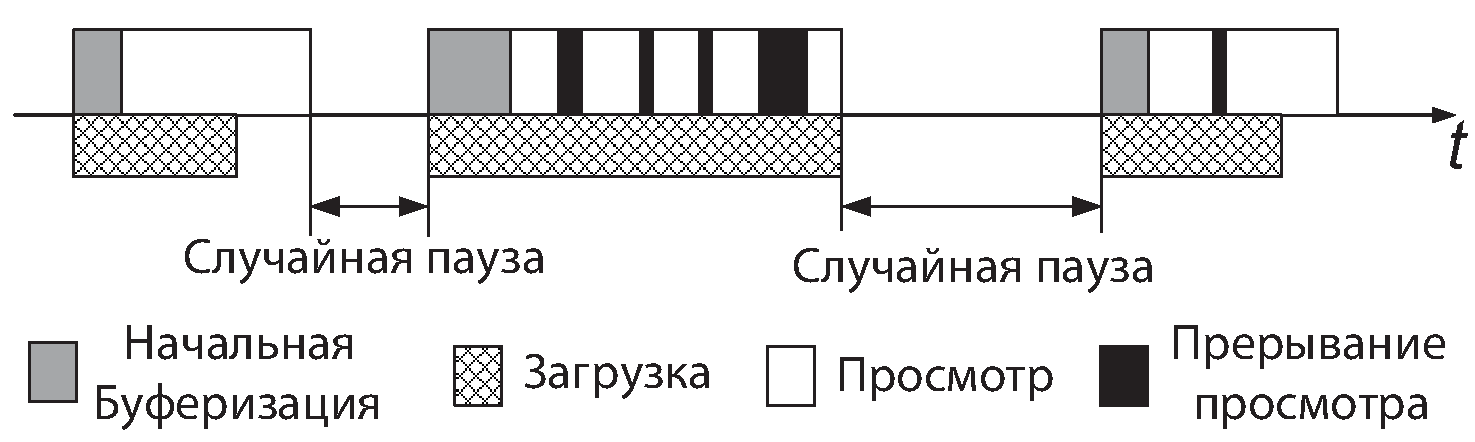
\includegraphics[width=\textwidth]{Chapter2/UeBehaviorModel.pdf}
\caption{Временная диаграмма поведения пользователя при просмотре видео}
\label{fig:UeBehaviorModel}
\end{center}
\end{figure}

Из модели поведения пользователя следует, что все время нахождения пользователя в системе можно разделить на три периода:
\begin{itemize}
	\item \textit{Буферизация}: пользователь ожидает начала или возобновления проигрывания видео (включает в себя начальные буферизации и прерывания воспроизведения, вызванные опустошением буфера);
	\item \textit{Просмотр}: штатное состояние, когда буфер на пользовательском устройстве достаточен и пользователь просматривает видеопоток;
	\item \textit{Пауза}: пользователь выбирает следующее видео для просмотра (в данном периоде просмотр и загрузка видео не осуществляются).
\end{itemize}
В дальнейшем будут использоваться конструкции $b_i^T$, $w_i^T$ и $p_i^T$ для обозначения общей длительности буферизации, просмотра и пауз пользователя $i$ за время в отрезке $[0, T]$.

\begin{definition}
\label{def:VideoSparseness}
    \emph{Коэффициент разряженности видеопотока пользователя $i$}~--~это отношение суммы длительностей просмотра и пауз к длительности просмотра пользователя $i$ за интервал времени $T\rightarrow\infty$:
    $$\gamma_i = \lim\limits_{T\rightarrow\infty} \frac{w_i^T + p_i^T}{w_i^T}.$$
\end{definition}
Данный коэффициент описывает насколько длительны паузы между просмотрами видео по сравнению с длительностью просмотра пользователя. Очевидным является факт, что значение $\gamma_i \geq 1, i=\overline{1,N}$.

Дальнейшее описание аналитической модели будет производится в порядке справа налево, в прямом соответствии с рисунком~\ref{fig:SystemModel}. Определим формат хранения и представления видеоинформации на удаленном контент сервере. Основываясь на информации, представленной подразделе~\ref{chap1:VideoFormat} на видео контент сервере все видео представляется в виде последовательности из сегментов равной длительности $d$ секунд. Длительность видеопоследовательностей на контент сервере является независимой случайной величиной $m$ распределенной по закону с конечными математическим ожиданием и дисперсией. Таким образом, для каждого пользователя существует средняя длительность просмотренных видео роликов: $M[m_i] = \overline{m}_i, i=\overline{1,N}$, где $m_i$~--~длительности заказанных роликов пользователем $i$.

Репрезентация каждой видеопоследовательности однозначно сопоставляется с битовой скоростью потока. Далее в работе, для обозначения битовой скорости потока, просматриваемого пользователем $i$, будет использоваться конструкция $R_i$. Все видеопоследовательности на контент сервере доступны в битовых скоростях в непрерывном отрезке от $R_{min}$ до $R_{max}$:
\begin{equation}
\nonumber
R_i \in [R_{min}, R_{max}], i=\overline{1,N}.
\label{eq:BitrateConstr}
\end{equation}
В реальной системе непрерывность битовых скоростей может быть достигнута использованием на удаленном сервере траскодеров видеопотока. Траскодер~--~программный комплекс, позволяющий в режиме реального времени получать видеопоток с заданной битовой скоростью из потока с более высокой битовой скоростью. Использование траскодирования видеопотока позволяет видеоплееру подбирать битовую скорость видео под конкретные условия системы передачи видеоданных. Общая структура и особенности работы траскодеров видеопотока описаны в работах~\cite{1184336,1369700}.

Далее определим модель магистральной сети передачи информации и опорной сети оператора. Исходя из анализа централизованных систем передачи видеоинформации следует, что магистральная и опорная сети обладают схожими характеристиками: высокая скорость передачи информации и низкая задержка, следовательно, являются высоко надежными и не вносят негативных эффектов при передаче видеоконтента (подраздел~\ref{chap2:WirelessSystemStructure}). В модели (рисунок~\ref{fig:SystemModel}) оба данных компонента сети были объединены в Магистральную сеть передачи информации.

Следующим шагом будут рассмотрены особенности работы радиосети и базовой станции. Модель радиосети является ключевой для предлагаемой модели, поэтому ее представление разделено на несколько пунктов:
\begin{itemize}
  \item Предварительный анализ;
  \item Модель беспроводного канала;
  \item Распределение ресурсов беспроводного канала.
\end{itemize}

Первым пунктом представляется предварительный анализ особенностей работы радиосети, целью которого ставится определение общего вида модели. Из описания в подразделе~\ref{chap2:CoreNetwork} следует, что вся зона обслуживания разделена на соты, в каждой из которых установлена базовая станция. В зависимости от географического положения абонента, пользовательское устройство подключается к определенной базовой станции. Базовые станции в различных сотах работают независимо друг от друга: невозможна ситуация, когда одно и тоже устройство обслуживают несколько станций одновременно, так же решение о выделении ресурсов беспроводного канала принимается независимо, от работы базовых станций в соседних сотах (подраздел~\ref{chap2:RadioNetwork}). Следовательно, каждую соту возможно рассматривать как отдельную независимую систему, в которой необходимо производить оптимизацию передачи видео. На основании вышеизложенного, далее в работе будет рассматриваться работа только одной соты.

Следующим пунктом будет представлена модель беспроводного канала передачи информации. Рассматриваемая модель предполагает, что пользователи в соте могут находится в различных условиях беспроводного канала, вызванные удаленностью от базовой станции. Последовательно рассмотрим восходящий и нисходящий беспроводные каналы. В современных централизованных системах связи восходящий канал обладает сравнимыми характеристиками с нисходящим, однако, его загруженность несравнимо меньше по сравнению с нисходящей линией связи. Как следствие, в предлагаемой модели восходящий радиоканал считается абсолютно надежным и задержкой передачи запросов на сегменты видео можно пренебречь.

Аналитическая модель уделяет большое внимание нисходящему каналу связи, так как от его производительности зависит удовлетворенность пользователей в соте. В данной работе рассматривается модель канала, обладающая следующим свойством: затухание при распространении сигнала происходит одинаково по всей ширине полосы передачи информации для конкретного пользователя в одном моменте времени. В реальной системе, основанной на стандарте LTE, данное допущение приводит к равенству оценок отношений сигнал/шум для всех ресурсных блоков в рамках одного подкадра конкретного пользователя. Следствием равенства отношений сигнал/шум для конкретного пользователя является равенства выбранных кодо-модуляционных схем и передаваемого объема информации для всех ресурсных блоков в подкадре.

Состояние беспроводного канала пользователя $i$ возможно охарактеризовать максимальной пропускной способностью канала.
\begin{definition}
\label{def:MaxThroughput}
    \emph{Максимальная пропускная способность канала пользователя $i$}~--~скорость передачи информации по беспроводному каналу, если все доступные ресурсы были выделены $i$-му пользователю.
\end{definition}
Это аналогично скорости получения данных при условии, что пользователь $i$ находится один в соте. Далее в работе, для обозначения максимальной пропускной способности пользователя $i$ будет использоваться конструкция $C_i$, а для сокращения текста слово <<максимальная>> будет опускаться.

Характеристики беспроводного канала передачи информации для каждого пользователя могут изменяться во времени, следовательно значение пропускной способности канала является случайным процессом: $C_i(t)$. Предполагается, что состояние беспроводного канала меняется медленно, таким образом, что в течении загрузки сегмента $j$ максимальная пропускная способность канала пользователя $i$ постоянна:
\begin{equation}
\nonumber
\left.C_i(t)\right\vert^{t_{i,j}+\Delta_{i,j}}_{t_{i,j}}=C_{i,j},
\label{eq:ChannelConst}
\end{equation}
где $t_{i,j}$~--~момент времени начала загрузки пользователем $i$ сегмента $j$, $\Delta_{i,j}$~--~длительность загрузки пользователем $i$ сегмента $j$, $C_{i,j}$~--~максимальная пропускная способность канала пользователя $i$ в течении загрузки сегмента $j$. Таким образом, значения $C_i(t)$ являются зависимыми случайными величинами.

Центральное положение в представляемой аналитической модели занимает алгоритм планирования распределения ресурсов беспроводного канала, установленный на базовой станции. Введем определение алгоритма планирования.

\begin{definition}
\label{def:SchedulingAlg}
    \emph{Алгоритм планирования}~--~это правило, в соответствии с которым базовая станция в момент времени $t$ распределяет доли ресурсов беспроводного канала $\alpha_i(t)$ для пользователя $i$.
\end{definition}

Таким образом, работу алгоритма планирования в момент времени $t$ возможно описать набором функций: ${A}(t) = \left\{\alpha_{i}(t), i = \overline{1,N}\right\}$. Очевидным ограничением на возможные значения функций $\alpha_i(t)$ является следующее неравенство:
\begin{equation}
\forall t: \sum\limits_{i=1}^{N}\alpha_{i}(t) \leq 1.
\label{eq:sumAlpha}
\end{equation}
Неравенство (\ref{eq:sumAlpha}) может быть интерпретировано следующим образом: в любой момент времени работы алгоритма планирования общий объем выделенных ресурсов не превышает доступного объема ресурсов для канала передачи информации. Следовательно, для любого пользователя $i$, мгновенная скорость передачи информации в нисходящем канале связи $S_i(t)$ может быть вычислена следующим образом:
\begin{equation}
S_i(t) = \alpha_i(t) C_i(t).
\label{eq:MomentRate}
\end{equation}

Алгоритм планирования в каждый момент времени решает задачу распределения ресурсов беспроводного канала. Для решения данной задачи ему доступна информация о предыстории, а именно доли выделенных ресурсов канала, значения пропускных способностей канала и объем переданной информации для каждого пользователя:
\begin{equation}
A(t) = \mathcal{A}\left( S_i(\tau), C_i(\tau);\tau<t, i=\overline{1,N} \right),
\label{eq:SchedulingRule}
\end{equation}
где $\mathcal{A}\left(\cdot\right)$ является алгоритмом планирования. В формуле (\ref{eq:SchedulingRule}) информация о предыстории выделенных долей беспроводного канала и объемах переданной информации для пользователя $i$ агрегированы в значении $S_i(\tau)$, так как данные параметры задаются соотношенем (\ref{eq:MomentRate}).

Важно отметить факт, что для планировщика базовой станции пользователь в каждый момент времени может находиться в одном из двух состояний: активном и неактивном. Пользователь считается активным, если у данного пользователя есть информация для передачи в нисходящем канале на базовой станции, иначе пользователь считается неактивным. В реальной системе, активность абонента так же определяется на основе заполненности очередей на RLC уровне (подраздел~\ref{chap2:RadioNetwork}). Основываясь на модели поведения пользователя при просмотре видео, пользователь может является активным только в период осуществления загрузки данных (рисунок~\ref{fig:UeBehaviorModel}). Однако, современные видеоплееры осуществляют паузы между заказами сегментов видео, и в течении данных пауз пользователь является неактивным для планировщика ресурсов беспроводного канала.

В данной диссертационной работе рассматриваются алгоритмы планирования, которые удовлетворяют представленному ниже набору свойств:
\begin{itemize}
	\item В каждый момент времени активному пользователю гарантировано выделение минимальной доли ресурсов канала $\alpha_{i}^{min}$:
	\begin{equation}
		\nonumber
		\begin{cases}
			\alpha_i(t) = 0, & \text{пользователь $i$ неактивен в момент времени $t$} \\
			\alpha_i(t) \geq \alpha_{i}^{min}, & \text{пользователь $i$ активен в момент времени $t$}\\
		\end{cases}.
	\end{equation}
	Минимальная доля ресурсов канала является величиной, отличной от нуля: $\alpha_{i}^{min} > 0$, и сумма минимальных долей ресурсов канала для всех пользователей не превышает общего объема ресурсов, доступных для планирования: $\sum\limits_{i=1}^{N}\alpha_{i}^{min} \leq 1$.
	\item Ресурсы беспроводного канала не могут быть выделены неактивному абоненту.
	\item В каждый момент времени планировщик распределяет все доступные ресурсы между активными абонентами:
	\begin{equation}
		\sum\limits_{i=1}^{N}\alpha_{i}(t) =
		\begin{cases}
			0, & \text{в момент времени $t$ все пользователи неактивны} \\
			1, & \text{иначе}\\
		\end{cases}.
	\end{equation}
\end{itemize}

В завершении будет определена модель видеотрафика и видиоплеера. В данной работе предполагается, что видеоплеер и видео контент сервер поддерживают технологию адаптивной передачи видеоконтента DASH (подраздел~\ref{chap1:VideoPlayers}) (рисунок~\ref{fig:PlayerModel}). Видеоплеер, установленный на пользовательском устройстве, осуществляет последовательную загрузку сегментов видеопоследовательности: следующий сегмент видео может быть заказан после окончания загрузки предыдущего и некоторой задержки. Пауза между заказами обусловлены стратегией наполнения буфера и моделью поведения пользователя. Данная задержка может быть короткой, если загружается сегмент в середине видео и достаточной длинной, если загружается первый сегмент, в случае если данная задержка включает в себя случайную паузы между просмотрами видеопоследовательностей, представленные на рисунке~\ref{fig:UeBehaviorModel}.

\begin{figure}[htbp]
\begin{center}
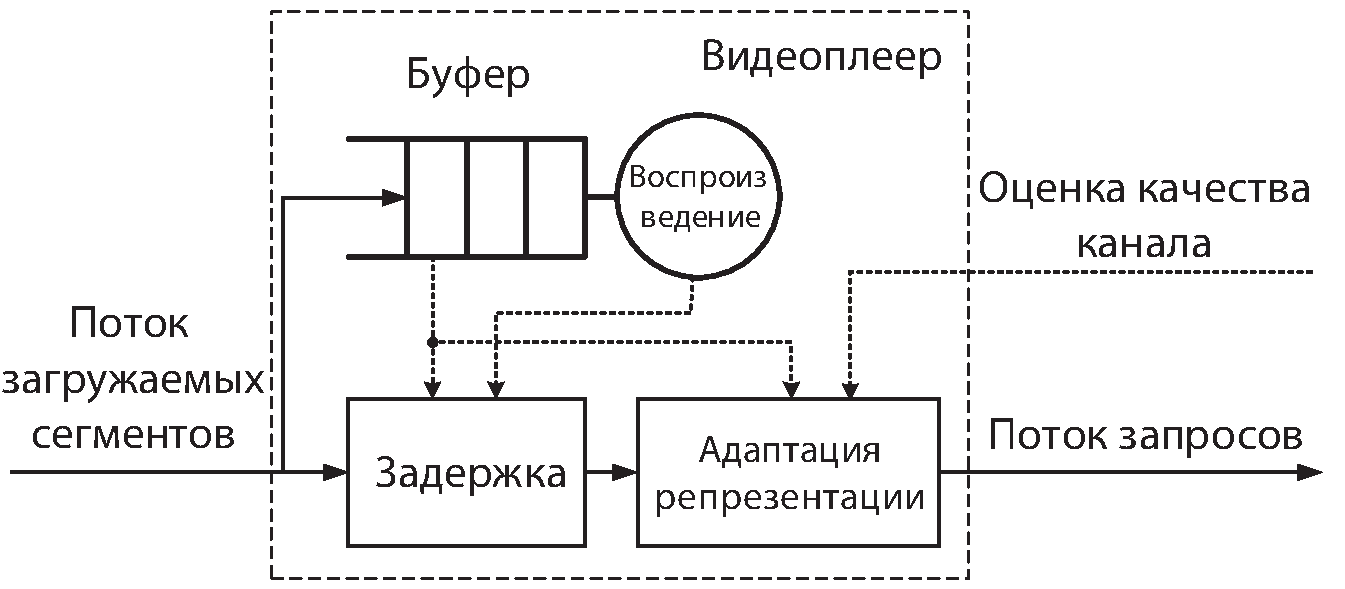
\includegraphics[width=\textwidth]{Chapter2/PlayerModel.pdf}
\caption{Модель воспроизводящего устройства}
\label{fig:PlayerModel}
\end{center}
\end{figure}

При заказе нового сегмента видеопоследовательности видеоплеер решает задачу выбора репрезентации для заказываемого сегмента. В предлагаемой модели репрезентация сегмента однозначно сопоставлена с битовой скоростью, таким образом задача выбора репрезентации сводится к задаче адаптации битовой скорости потока. Для решения данной задачи видеоплеер может использовать информацию о наполненности буфера и других статистиках: оценку скорости получения информации в течении предыдущих сегментов, информацию о качестве беспроводного канала и т.д. Задача адаптации битовой скорости потока может быть представлена следующим выражением:
\begin{equation}
\nonumber
R_{i,j} = \mathcal{B}\left(R_{i,k}, C_i(\tau), S_i(\tau); k < j, \tau<t_{i,j} \right),
\end{equation}
где $\mathcal{B}\left(\cdot\right)$ является функцией вычисления битовой скорости $j$-го сегмента пользователя $i$, $R_{i,j}$~--~битовая скорость потока $j$-го сегмента пользователя $i$.

Очевидным является факт, что частое переключение битовых репрезентаций негативно влияет на качество восприятия видеопотока: в некоторых случаях быстрое переключение репрезентаций при просмотре приводит к проявлению симптомов неврологических расстройств. Поэтому в современных реализациях видеоплееров количество переключений в единицу времени ограничено сверху~\cite{widash}. Обычно адаптация видеопотока под конкретные условия беспроводного канала происходит в короткий промежуток времени в начале загрузки нового видео. Таким образом, если существуют математическое ожидание: $E[R_i] = \lim\limits_{j \rightarrow \infty}E[R_{i,j}]$ и среднее квадратичное отклонение: $\sigma\left[R_{i}\right] = \lim\limits_{j \rightarrow \infty}\sigma\left[R_{i,j}\right] $ битовой скорости просматриваемого потока, то коэффициент вариации битовой скорости видеопотока ограничен сверху некоторой константой, значение которой зависит от типа и настроек видеоплеера:
\begin{equation}
\forall i: \frac{ \sigma\left[R_{i}\right] }{ E\left[R_{i}\right]} \leq \nu^R_i.
\label{eq:SwitchRatio}
\end{equation}

Введение модели видеоплеера завершает представление аналитической модели. Обобщая описанное выше, предлагается следующая система допущений для аналитической модели передачи видеоинформации в централизованных беспроводных сетях.
\begin{itemize}
	\item \textit{Формат представления видеоинформации}:
	\begin{itemize}
		\item Все видеопоследовательности разбиты на сегменты одинаковой длительности $d$ секунд;
		\item Все видеопоследовательности на видео контент сервер представлены в непрерывном отрезке битовых скоростей: \mbox{$R_i \in [R_{min}, R_{max}], i=\overline{1,N}$};
		\item Длительности видеопоследовательностей $m$, представленных на видео сервере, является независимыми случайными величинами с конечными математическим ожиданием и дисперсией.
	\end{itemize}
	\item \textit{Общие характеристики сети передачи информации}:
	\begin{itemize}
		\item Задержка в восходящем канале считается пренебрежимо малой, и загрузка сегментов видеоданных начинается незамедлительно в момент отправки запроса.
	\end{itemize}
	\item \textit{Модель поведения пользователя при просмотре видео}:
	\begin{itemize}
		\item Паузы между просмотрами $\tau_i$ является независимыми случайными величинами с конечными математическим ожиданием ($\overline{\tau}_i$) и дисперсией.
	\end{itemize}
	\item \textit{Модель беспроводного канала}:
	\begin{itemize}
		\item Затухание при распространении сигнала происходит одинаково по всей ширине полосы передачи информации для конкретного пользователя в одном моменте времени;
		\item В течении загрузки сегментов видео максимальная пропускная способность канала постоянна: $\left.C_i(t)\right\vert^{t_{i,j}+\Delta_{i,j}}_{t_{i,j}}=C_{i,j}$;
		\item Последовательность случайных величин $C^{-1}_{i,1}, C^{-1}_{i,2}, \ldots$ обладает конечным математическим ожиданием и конечным коэффициентом вариации $\nu^{C}_i$.
	\end{itemize}
	\item \textit{Модель планировщика ресурсов беспроводного канала}:
	\item \textit{Модель видеоплеера}:
\end{itemize}


\section{Выводы по разделу}